%% This is an example first chapter.  You should put chapter/appendix that you
%% write into a separate file, and add a line \include{yourfilename} to
%% main.tex, where `yourfilename.tex' is the name of the chapter/appendix file.
%% You can process specific files by typing their names in at the 
%% \files=
%% prompt when you run the file main.tex through LaTeX.
\chapter{Macrostates}

As discussed in Chapater \ref{pfChapter}, there is signficant
motivation to not think of RNA as a typical energy minimizing
system. A ball rolls to the bottom of a valley, if it is
smooth. However, the energy landscape of RNA is shallow and bumpy: the
deepest point (MFE) can be around $10^{-10}$ times the total partition
function, with many local minima for example in Figure
\ref{fig:localMinima}. In 2005, Ding and Lawrence showed that the
Boltzmann distribution for RNA naturally parititions into distinct
clusters \cite{ding2005rna} as seen in Figure
\ref{fig:centroidFig}. Therefore, it is better to think of RNA as a
thermodynamic system in equilibrium between several different
macrostates, defined:
\begin{figure}[t]
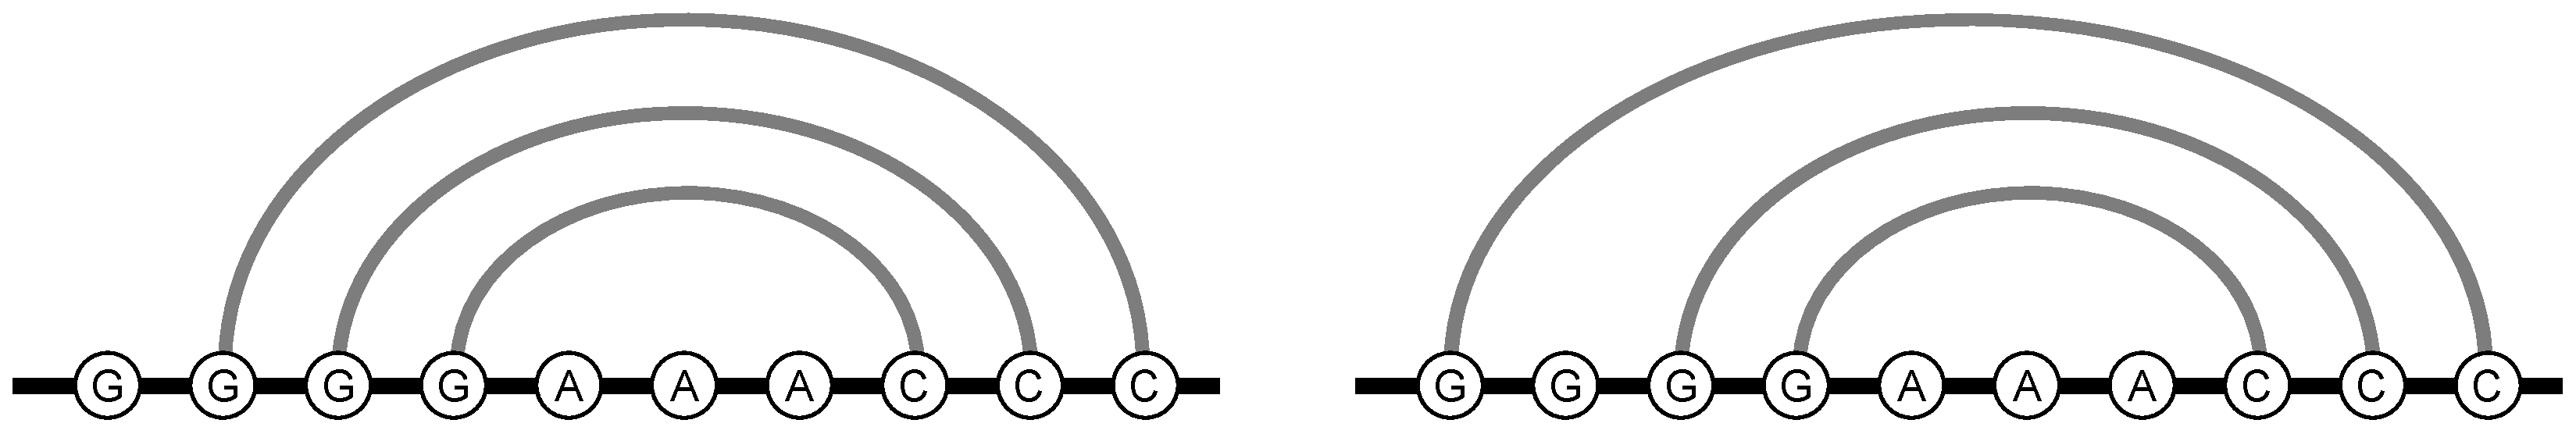
\includegraphics[width=\textwidth]{multi-minima.eps}
\caption{Here are two local minima of the same strand,
  ``GGGGAAACCC''. To get from one to the other, the outermost bond
  must be broken, raising the energy. There are multitudes of such
  local minima, and this contradicts any idea of a ``smooth'' decent
  to the global minimum.}
\label{fig:localMinima}
\end{figure}
\begin{description}
\item[Macrostate:] a set of states of RNA containing similar
  structural qualities, or within some metric of energy distance from
  each other.
\end{description}
The defintion of Macrostate is left vague, because there currently is
no widespread agreement on how to identify and classify them. If the
set of states defining a macrostate is $S$, then the probability of a
macrostate is defined as
\begin{equation} 
P(S) = \sum_{s \in S} P(s).
\end{equation}
This can be thought of as integrating ``infinitesimals'' ($P(s)\ll Z$)
over an energy ``basin''.

In the past 10 years, several groups have started to explore this
concept. There are two approaches, in general, to define basins and
classify structures into them. The first class of methods defines the
basins from the top-down: given a number of stochastically sampled
structures, we divide them into groups based on some kind of distance
metric. These methods tend to be very similar to typical clustering
algorithms used in computer science and data analysis.

Another approach is to start at local minima and climb up the energy
barriers between minima. These methods can be used to accurately
compute the energies of the transition states between local minima and
these can tell you the kinetics of the structure. This method was
devloped by the makers of ViennaRNA and continues to be a main area of
research \cite{PhysRevE.83.011113} \cite{wolfinger2004efficient} .

In general, finding macrostates, estimating their size and where they
overlap will tell you the probability of that macrostate and the
transition probabilities between them. This information provides a
much greater understanding of the function of an RNA strand than
standard minimum free energy analysis. 

\section{Sfold}

The author's of the stochastic traceback paper
\ref{ding2003statistical} Ding and Lawrence explored clustering the
results of their algorithm and found that it not only improved the
prediction accuracy \ref{ding2005rna}, but indicated that there should
be a revolutionary change of perspective in terms of the mechanics of
RNA. Specifically they found that 45\% of sequences they studied did
not have the MFE in the biggest, most probable cluster. If the MFE is
not in the most probable cluster, any predictions based on the MFE for
that strand are going to be inaccurate. They confirmed this and found
that the MFE predictions perform the worst in these kinds of
strands. Another important finding was that in 45\% of sequences do
not have a macrostate with greater than 70\% probability, but that
most sequences do not have more than 3 or 4 clusters. If this is true,
this means that there must not be a single dominant structure for that
RNA strand, but rather that it is in equilibrium between macrostates,
and these different states and the transitions between them have
critical biological roles. 

Ultimately the change in perspective to clustering analysis improved
the results of their prediction. They compared their results to
secondary structures that have been determined by comparative sequence
analysis and looked at the results for the MFE, the biggest cluster,
and the cluster that performed the best. The biggest cluster centroid
and the best cluster centroid beformed better than the MFE in 74.1\%
and 91.4\% of sequences, respectively, where performance was measured
by their base pair distance metric from the comparative sequence
structure (see Sfold Methods) \cite{ding2005rna}
\cite{mathews2006revolutions}. The centroids also had less errors in
measures such as the positive predictive value (PPV), defined as the
rate of true positives, improving to up to 30\% in the best cluster
centroid. One interesting finding they found was that the natural
sequence found by comparative sequence analysis was not necessarily in
the biggest cluster. This could be because the strand is not
necessarily in thermal equilibrium, rather assembles itself in a
macrostate that is easily accessible from the unfolded state (low
energy barrier) but that has not as much access to the most Boltzmann
probable macrostate (high energy barrier). This puts even more
emphasis on knowing the transition energies between states.

\subsection{Sfold Methods}
\begin{figure}[t]
\bf The algorithm starts with structures all in the same cluster and
repeats the following sequence:
\begin{enumerate}
\item Find the structure $s_m$ with highest average distance
  $D(s_m,s_n)$ for all $s_n$ in the same cluster and create a new
  cluster containing just $s_m$.
\item For each structure $s_n$ that is closer to $s_n$ than the rest
  of the structures on average, add it to the cluster containing $s_m$.
\item For the 2 new clusters created by this algorithm, unless
  stopping criterion has been met, repeat this algorithm on each. 
\end{enumerate}
Stopping criteria:
CH-index $$CH(k)=\frac{B(k)/(k-1)}{W(k)/(n_{total}-k)}$$ is maximized,
where $k$ is the number of clusters, $B(k)$ is between-cluster sum of
squares, $W(k)$ is average in-cluster sum of squares, and $n_{total}$
is the total number of structures.
\caption{The DIANA algorithm for dividing data into clusters based on
  a distance measure $D$. Used by Sfold to divide structures into
  macrostates.}
\label{fig:diana-pseudocode}
\end{figure}

Sfold clusters RNA structures that have been stochastically sampled
according to their Boltzmann probabilities using the DIANA clustering
algorithm, using a base pair metric as the distance. Defining
$I_{ij}^m$ to be a binary value that is 1 if secondary structure $s_m$
contains the base pair $(i,j)$ and 0 otherwise, the metric is defined
as
\begin{equation}
D(s_m, s_n) = \sum_{j,k} (I^m_{jk} - I^n_{jk})^2,
\end{equation}
or roughly adding 1 for every base pair that $s_m$ and $s_n$ do not
share. Using this distance metric, the DIANA clustering goes as
described in Figure \ref{fig:diana-pseudocode}, budding off structures
by finding the most different structure, and tries to maximize the
ratio of between average between-cluster distance and average
in-cluster distance.

The cluster centroids, $s_s$, are found within each cluster created by
DIANA analysis by creating an upper-triangle matrix $I^s_{jk}$ that
solves the linear program:
\begin{equation}
\begin{array}{ll@{}ll}
\text{minimize}  &\displaystyle\sum_{m} D(s_s, s_m)\  =&\ \displaystyle\sum_{m,i,j}( I^m_{ij} - I^s_{ij})^2 \\
\text{subject to}& I^s_{ij} + I^s_{kl} \leq 1    & \forall (i < k\ \&\ k < j) \\
                                                              & I^s_{ij} \in \{0, 1\} & \forall i,j. &
\end{array}
\end{equation}
[TODO: should I delete and just say ``solve a linear program''?]
This produces a valid structure that is as close as possible to the
other structures in the cluster. 

\subsection{Drawbacks}

While the base-pairs distance metric is useful and efficient from a
computer science standpoint, a better distance measure would be based
on the energy cost to get from one structure to the other. Then
distances could be related to other thermodynamic variables, such as
time constants of transitions, and would be a more physically based
method of determining energy states. While base-pair differences are
related to the energy needed to go from one structure from another,
they do not directly correspond and so can lead to some slight
discrepencies. In their paper \emph{Comparing RNA secondary structures
  using a relaxed base-pair score}, Agius, Bennet, and Zuker examine
how it is possible to construct 3 secondary structures for the strand
where the last 2 are the same base-pair distance from the first but
one looks similar and the other is very different. They go on to
develop a different distance metric they call \emph{relaxed-base-pair}
\cite{agius2010comparing}. Aalberts and Jannen developed another way
of measuring distance, explained in the Nestor section. 

One other drawback is that there is no good way of measuring the
transition state between two macrostates. The way the clustering
algorithm works allows for no ``in between''. The PF clustering
method, a slight modification of the Nestor algorithm, allows both a
better distance metric and an ability to measure transtition
states. Another method, which deserves mentioning in my opinion, was
developed by the team of ViennaRNA, which they called Barriers.

\section{Vienna RNA: Barriers}

Barriers is a tool designed by those behind the software package
ViennaRNA to compute macrostates by starting at individual local
minima and climbing up the free energy basins by making and breaking
pairs \cite{flamm2002barrier}
\cite{wolfinger2004efficient}. Macrostates are thereby defined as the
set of states with the same local minima. This climbing is done by
using a physically accurate stochastic simulation, and this allowed
them to compute the transition probabilities between macrostates by
examining the probability of transitioning from a state with one local
minima to a state with another local minima. Here I will be following
the results of their most recent work, \emph{Efficient exploration of
  discrete energy landscapes} by Mann and Klemm (2011) and
\emph{Memory-efficient RNA energy landscape exploration} by Mann
\emph{et al} (2014) \cite{PhysRevE.83.011113} \cite{mann2014memory},
where they develop a clear and precise formalism.

\subsection{Algorithm}

The algorithm uses the Metropolis-Hastings framework for simulating
the thermal process of RNA using a markov chain
\cite{metropolis1953equation} \cite{hastings1970monte}. Specifically, they define the energy
landscape of RNA to be a triple $(X, E, M)$ where
\begin{itemize}
\item $X$ is a finite set of states,
\item $E: X \to R$ is an energy function on $X$ (the Turner model),
\item $M: X \to \mathcal{P}(X)$ is a neighborhood function that
  assigns to each state $x \in X$ the set of states that could be
  reached from $x$ by breaking and making a single pair and including
  $x$ itself. $\mathcal{P}(X)$ is the power set of $X$.
\end{itemize}
\begin{figure}[t]
\bf The algorithm starts by ``seeding'' $n$ minima from $X$ using Ding
and Lawrence's stochastic traceback algorithm and then a gradient
decent using $M$. From there, for each state $x$:
\begin{enumerate}
\item Find basin $b = B(x)$ (trivial on first step).
\item Update the thermodynamic variables (see equations \ref{eq:Zb}
  and \ref{eq:Zbc}):
\begin{enumerate}
\item $Z = Z + w(x)$
\item $Z_b = Z_b  + w(x)$
\item For each $y \in M(x)$: $Z_{\{b, B(y)\}} = Z_{\{b, B(y)\}} +  \min \left (\frac{ w(y)  | M(x) |}{| M(y) |} , w(x) \right )$
\end{enumerate}
\item Find next state $y$ by sampling uniformly from $M(x)$ and
  accepting $x=y$ according to probability 
  $$p_{x\to y} = \min \left (\frac{w(y)|M(x)|}{w(x)|M(y)|},1\right
  ),$$ (equation \ref{eq:detailedBalance}), otherwise $x$ stays the
  same.
\item Go to step 1, unless sufficiently satisfied.
\end{enumerate}
Results: Probability of any macrostate $b$ is $Z_b/Z$, transition
probability from state $b$ to $c$ is $Z_{\{b, c\}}/Z_b$.
\caption{The algorithm by Flamm \emph{et al} as it appears in the most
  recent papers. Estimating macrostate probabilities and transition
  probabilities by direct stochastic simulation. Notation:
  $w(x)=e^{-E(x)/RT}$, $B(x)$ is the local minima found from $x$ by
  doing gradient descent on $M$.}
\label{fig:barriersAlgorithm}
\end{figure}
The algorithm is described as in Figure
\ref{fig:barriersAlgorithm}. Local minima are found from a stochastic
sample of the Boltzmann distribution. These minima are then used as
the starting points of markov chains generated by the Metropolis
algorithm. Specifically given a structure $x$, a structure $y$ is
chosen by uniformly sampling from $M(x)$, and that structure is
accepted as the next state of the chain with probability 
\begin{equation}
p_{x\to y} = \min \left ( \frac{ P(y) T(y \to x)}{ P(x) T(x \to y)} , 1 \right ) =  \min \left ( \frac{ e^{-E(y)/RT}  | M(x) |}{ e^{-E(x)/RT} | M(y) |} , 1 \right ),
\label{eq:detailedBalance}
\end{equation}
where $P(x)$ is the standard Boltzmann probability of the state $x$,
$e^{-E(x)/RT}/Z$, and $T(x \to y)$ is the probability of generating
the transition from $x$ to $y$, which is $1/|M(x)|$ because we
uniformly chose from $M(x)$. If the new state is not accepted, $x$ is
kept as the next state in the chain. Equation \ref{eq:detailedBalance}
fulfills the requirements of ``detailed balance'' which ensures that
the states of the markov chain will converge to the distribution
$P(x)$ according to Metropolis \emph{et al} and Hastings
\cite{metropolis1953equation} \cite{hastings1970monte}. 

For each state sampled in this manner we can compute it's local minima
and compute the thermodynamic variables of that basin on the fly. Let
$B \subset \mathcal{P}(X)$ be the set of all macrostates on the free
energy landscape. For an individual basin $b \in B$, we can define the
probability of the basin as:
\begin{equation}
P(b) = \sum_{x \in b} \frac{e^{-E(x)/RT}}{Z} = \frac{Z_b}{Z}, 
\end{equation}
where
\begin{equation}
Z_b = \sum_{x \in b} e^{-E(x)/RT}
\label{eq:Zb}
\end{equation}
is a quantity we can continuously update as the sample more states
$x$. We can additionally now define a quantity
$P_b(x)=e^{-E(x)/RT}/Z_b$ which is the probability of state $x$ within
basin $b$.
To compute the transition probabilities between two basins $b$ and $c$,
$q_{b \to c}$ and $q_{c \to b}$, we simply use a weighted sum of the
probabilities of transitioning from states in one to the other (using
shorthand $w(x)=e^{-E(x)/RT}$):
\begin{equation}
\begin{split} 
q_{b \to c} &= \sum_{x \in b} \left ( P_b(x) \sum_{y \in M(x) \cap c} p_{x \to y} \right ) 
\\ & = \sum_{x,y} \frac{w(x)}{Z_b} \min \left (\frac{ w(y)  | M(x) |}{ w(x)  | M(y) |} , 1 \right )
\\ & = Z_b ^{-1}\sum_{x,y}  \min \left (\frac{ w(y)  | M(x) |}{| M(y) |} , w(x) \right )
\\ & = Z_b^{-1} Z_{\{b, c\}},
\end{split}
\end{equation}
defining a new quantity
\begin{equation}
Z_{\{b, c\}} = \sum_{x \in b} \sum_{y \in M(x) \cap c} \min \left ( \frac{w(y) |M(x)|}{|M(y)|}, w(x) \right ). 
\label{eq:Zbc} 
\end{equation}
Notice that both the quantities $Z_b$ and $Z_{\{b, c\}}$ can be
updated with each new state $x$, as done in Figure
\ref{fig:barriersAlgorithm}. At the end of the computation, the
probabilities of each macrostate $b$ can be computed by the term
$Z_b/Z$, and the transition probability from $b$ to $c$ is
$Z_{\{b,c\}}/Z_b$. 

\subsection{Coarse Graining}

One of the drawbacks of Barriers is that there are a great many local
minima in the landscape of RNA, as shown in Figure
\ref{fig:localMinima}. To get good estimates of the thermodynamic
variables for each of the basins, the algorithm will exibit a very
long convergence time since very many states need to be sampled. One
way to combat the multiplicity of local minima is to use on of the
results of Ding and Lawrence, which is that they observed at maximum 3
or 4 major clusters in the landscape. Similar states with low energy
barriers ($q_{b \to c}$ is very high) can be merged into one
macrostate, the new thermodynamic parameters can just be added
($Z_{a=b\cup c}=Z_b+Z_c$, $Z_{\{a,d\}}=Z_bZ_{\{b,d\}}+Z_cZ_{\{c,d\}}$)
since each macrostate is disjoint by definition, this is called
coarse-graining and was implemented in Barriers as well.

\section{Nestor and RNAbows}

There are seperate clustering methods developed in published and
unpublished work by Aalberts and Jannen based on the concept of
non-nestedness \cite{aalberts2013visualizing}
\cite{aalbertsNestor}. Non-nestedness is a measure of how much
crossing there is between pairs of structures. Non-nestedness is a
physically based measure, since to get from one state to another, they
will have to break at least all non-nested pairs. Clustering analysis, similar to
the analysis done in Sfold can be done with this measure of distance.

To be precise, non-nestedness can be defined either in a sampled
ensemble or on partition function data. The partition function version
was developed as part of this thesis and will be explored in the next
section. For the former, large numbers of sequences are sampled using
the stochastic traceback algorithm. The probability of each pair
$P_{ij}$ is computed by counting the occurence in each strand in the
ensemble. Then the non-nestedness between two ensembles $\mu$ and
$\nu$ is defined as:
\begin{equation}
\Psi^{\mu\nu} = \sum_{k,l} \sum_{m,n \times (k,l)} P^{\mu}_{kl}
P^{\nu}_{mn},
\end{equation}
where $m,n \times (k,l)$ denotes the pairs $(m,n)$ that \emph{cross}
$(k,l)$. 

\subsection{Algorithm}

The goal of the algorithm is to find the most non-nested pair in the
ensemble, or $(k,l)$ such that
\begin{equation}
\max_{k,l} \sum_{m,n \times (k,l)} P^\mu_{kl}P^\nu_{mn}
\end{equation}
and then split the ensemble into an ensemble that includes
that pair and an ensemble that forbids that pair. This splitting is
continued recursively until chosen stopping rules have been
fulfilled. A standard stopping rule, one that is currently used in the
(unpublished) software is to set a number of output clusters desired,
preferrably a power of 2. 

The probability of each output cluster is simply the number of sampled
structures contained within it divided by the total number of sampled
structures. Unfortunately, similar to Sfold, there is no way to
estimate the transition states for the divided clusters. However the
PF version of Nestor can measure transition states as well as give
exact probabilities for macrostates, something that Nestor cannot do
because of statistical error. In this way the PF method is an
improvement over the stochastic method of Nestor.

\subsection{Visualization}
\begin{figure}[t]
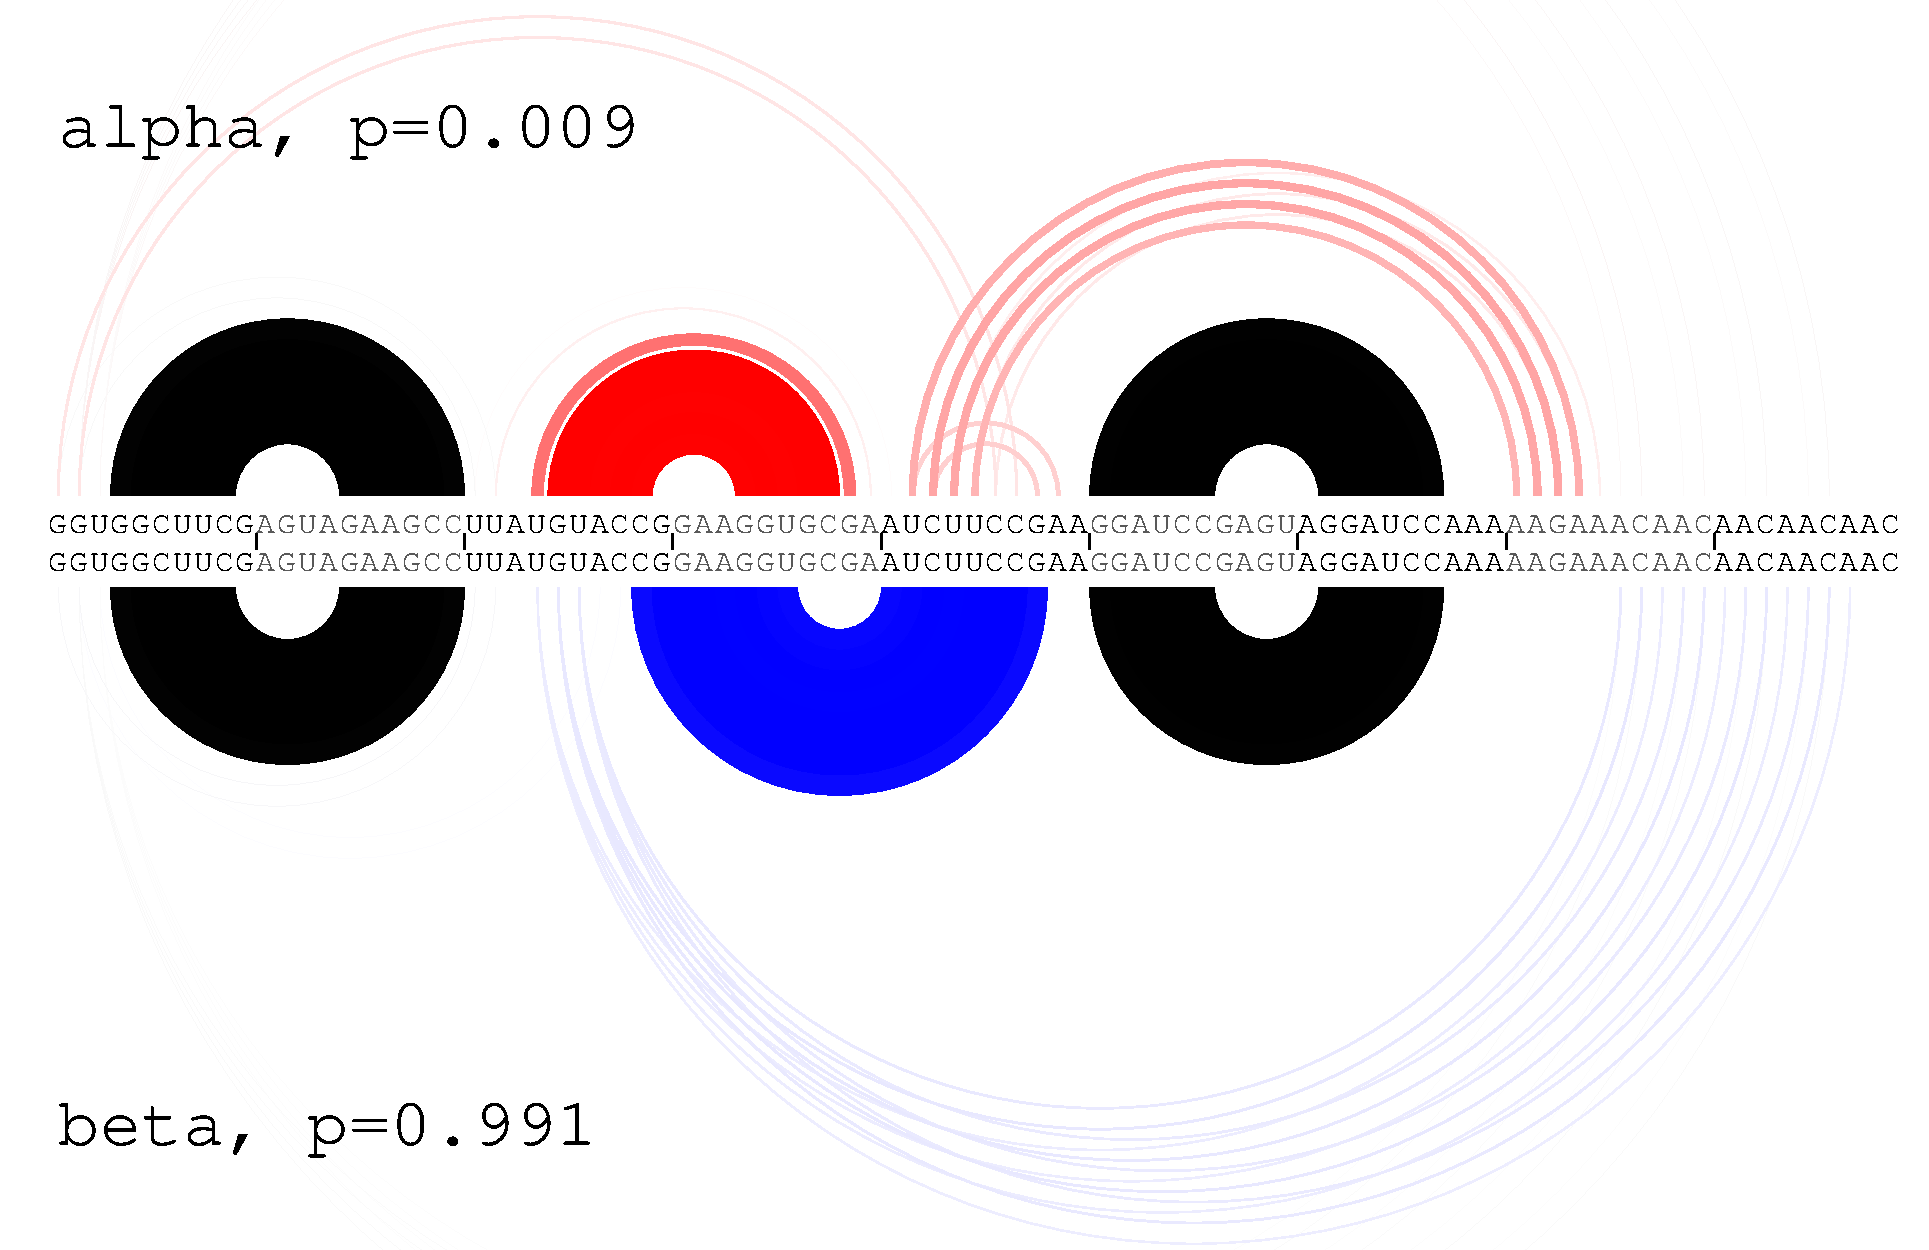
\includegraphics[width=\textwidth]{cluster_mstable.eps}
\caption{An RNAbow of the two main clusters of a strand of RNA. The
  two colors denote the two differnt clusters, and how solid the
  colors of the arcs are indicates how probable that base pairing
  is. The bottom sequence dominates the top sequence with 99\%
  Boltzmann probability. However, if the structure starts in the red
  state, it might require some energy to get to the blue state. The
  two ensembles are most non-nested in the middle region, and in order
  to get from one to the other one must at least break every pair
  where the red heavy stem crosses the blue heavy stem.}
\label{fig:rnaBow}
\end{figure}

A nice method of visualizing and comparing two different subensembles
is implemented in RNAbows. RNAbows takes in two different ensembles
and calculates pairs info about each. Each subensemble is given a
color, and circular arcs are drawn in between pairs of bases, where
the color and alpha is weighted by their probability. Bases that are
shared between the two ensembles are colored black. An example of an
RNAbow is in Figure \ref{fig:rnaBow}.

\section{PF method}
\begin{figure}[t]
\center
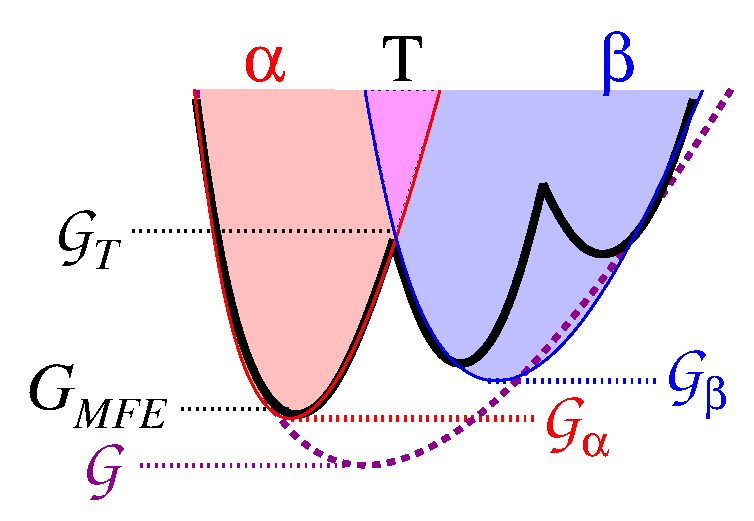
\includegraphics[width=.3\textwidth]{WLandscape.eps}
\caption{What we try to isolate in Nestor. The largest basins are
  identified by identifying the most non-nestedpair. These basins
  might contain several ViennaRNA-Barriers-type basins. The top down
  approach lets us look at the most important basin/clusters
  efficiently.}
\label{fig:landscape}
\end{figure}

The PF method is really just a small modification of the Nestor
algorithm. Instead of using a sampled ensemble of states, we compute
the partition function and its associated matrices $Q(i, j)$ and
$Q^b(i,j)$. The probability of a pair can be computed from a pretty
complicated formula given in McCaskill's paper
\cite{mccaskill1990equilibrium} [TODO: find the better formula and
  substitute]:
\begin{equation}
P(h,l) = \frac{Q(1, h-1) Q^b(h,l) Q(l+1, n)}{Q(1, n)} + \text{ ... overhead terms}
\end{equation}
From here we can find the most non-nested pair in this ensemble. Once
we have obtained this pair $(h, l)$ we can compute an ensemble with
all the pairs crossing $(h, l)$ restricted. From there we have an
ensemble $\mu$, which contains the structures nested with $(h,l)$. To
compute the other ensemble $\nu$, we ``flip'' the probabilities of $\mu$
with the formula
\begin{equation}
P_{i,j} = p^\mu P^\mu_{ij} + p^\nu P^\nu_{ij},
\end{equation}
where $p^\mu$ is the macrostate probability of $\mu$ and $P^\mu_{ij}$
is the probability of the pair $(i,j)$ occuring withing macrostate
$\mu$. Noting that we can approximate $p^\nu = 1 - p^\nu$, we have
that
\begin{equation}
P^\nu_{ij} \approx \frac{P_{ij} - p^\mu P^\mu_{ij}}{1 - p^\mu}.
\end{equation}
These would be an equality if $\mu$ and $\nu$ were completely
disjoint, however we know there is an overlap region between them that
corresponds to the transition state. To estimate this transition
state, we can recompute the partition function for the ensemble under
the assumption that pairs with very small estimated $P^\nu_{ij}$ will
not occur, so we restrict these pairs. This new partition function
computation gives us the exact $P^\nu_{ij}$s. From here, we know the
probability of each macrostate is simply the partition function for
that macrostate divided by the original partition function
$Z_\mu/Z$. We can also estimate the transition probability by the
amount of overlap between the two states:
\begin{align}
Z_{\{\mu,\nu\}} &= Z_\mu + Z_\nu - Z, \\
P( \mu \to T) &= \frac{Z_{\{\mu,\nu\}}}{Z_\mu}, \\
P( \nu \to T) &= \frac{Z_{\{\mu,\nu\}}}{Z_\mu},
\end{align}
where $T$ is the transition state. Notice that the transition states
are defined slightly differently than Barriers because we have defined
that macrostates slightly differently. These probabilities can be used
to estimate the energy gap needed to be crossed in order to get from
one state to another, and can also be used as an automatic stopping
rule to be used instead of just explicity stating the number of
splits.

\section{Testing Nestor PF predictions using SHAPE experiments}

It would be very good to verify all these predictions against real
world experiments.  This is not as straightforward as it sounds, as
the Williams students who take Applications of Quantum Mechanics learn
for example, a lot of care must be taken to ensure that a single
photon experiment actually has one photon going through at a time. For
a theoretical biologist this task is exascerbated by the environment
in which the most important measurements must take place: inside
living things. For example, the partition function of an rna strand
describes its statistical properties in thermal equilibrium. However,
the living cell is certainly not in thermal equilibrium. Furthermore,
most measurements of RNA structure necessarily take RNA out of its
natural environment in order to examine it. 

Selective 2'-hydroxyl acylation analyzed by primer extention (SHAPE)
experiments have shown great potential in showing highly accurate
profiles of base-pairing in diverse solvent environments
\cite{wilkinson2006selective}. A colloquial description of these
experiments would be as follows: polymers are prepared that bind to
RNA at unpaired regions and an enzyme is added that cuts the the
polymers to lengths that are proportional to the index of the base
that they are bound to. These polymers are then strained using gel
electrophoresis which causes different length polymers to seperate
from one another. The counts of polymers at different lengths reveal
which bases are unpaired along the secondary structure of the
strand. This information can be used to inform standard secondary
structure algorithms, and was implemented by Katherine Deigan, David
Mathews, and Kevin Weeks in the RNAStructure package as an additional
energy term and saw accuracy improve up to 96-100\%
\cite{deigan2008accurate}.

\subsection{Mutate and Map experiments}

The experimental methods used to test our theoretical results were
those recently established by Das Lab at Stanford called ``mutate and
map'' experiments \cite{kladwang2011two}. The group recognized that
RNA exists in equilibrium between macrostates and attempted to
experimentally examine these states by disrupting pairs through
mutation. Specifically, for a sequence $n$ nucleotides long, Das Lab
produced $n+1$ sequences, sequence 0 being the normal sequence, 1
being the sequence with base 1 flipped to its opposite pair, 2 the
sequence with base 2 flipped to its opposite pair, all the way up to
sequence $n$ with base $n$ flipped to its opposite pair. Das Lab then
performed shape analysis on each of these strands and found which
bases were paired and unpaired. An example of a mutate and map
experimental output is in Figure \ref{fig:heatmap}.
\begin{figure}[t]
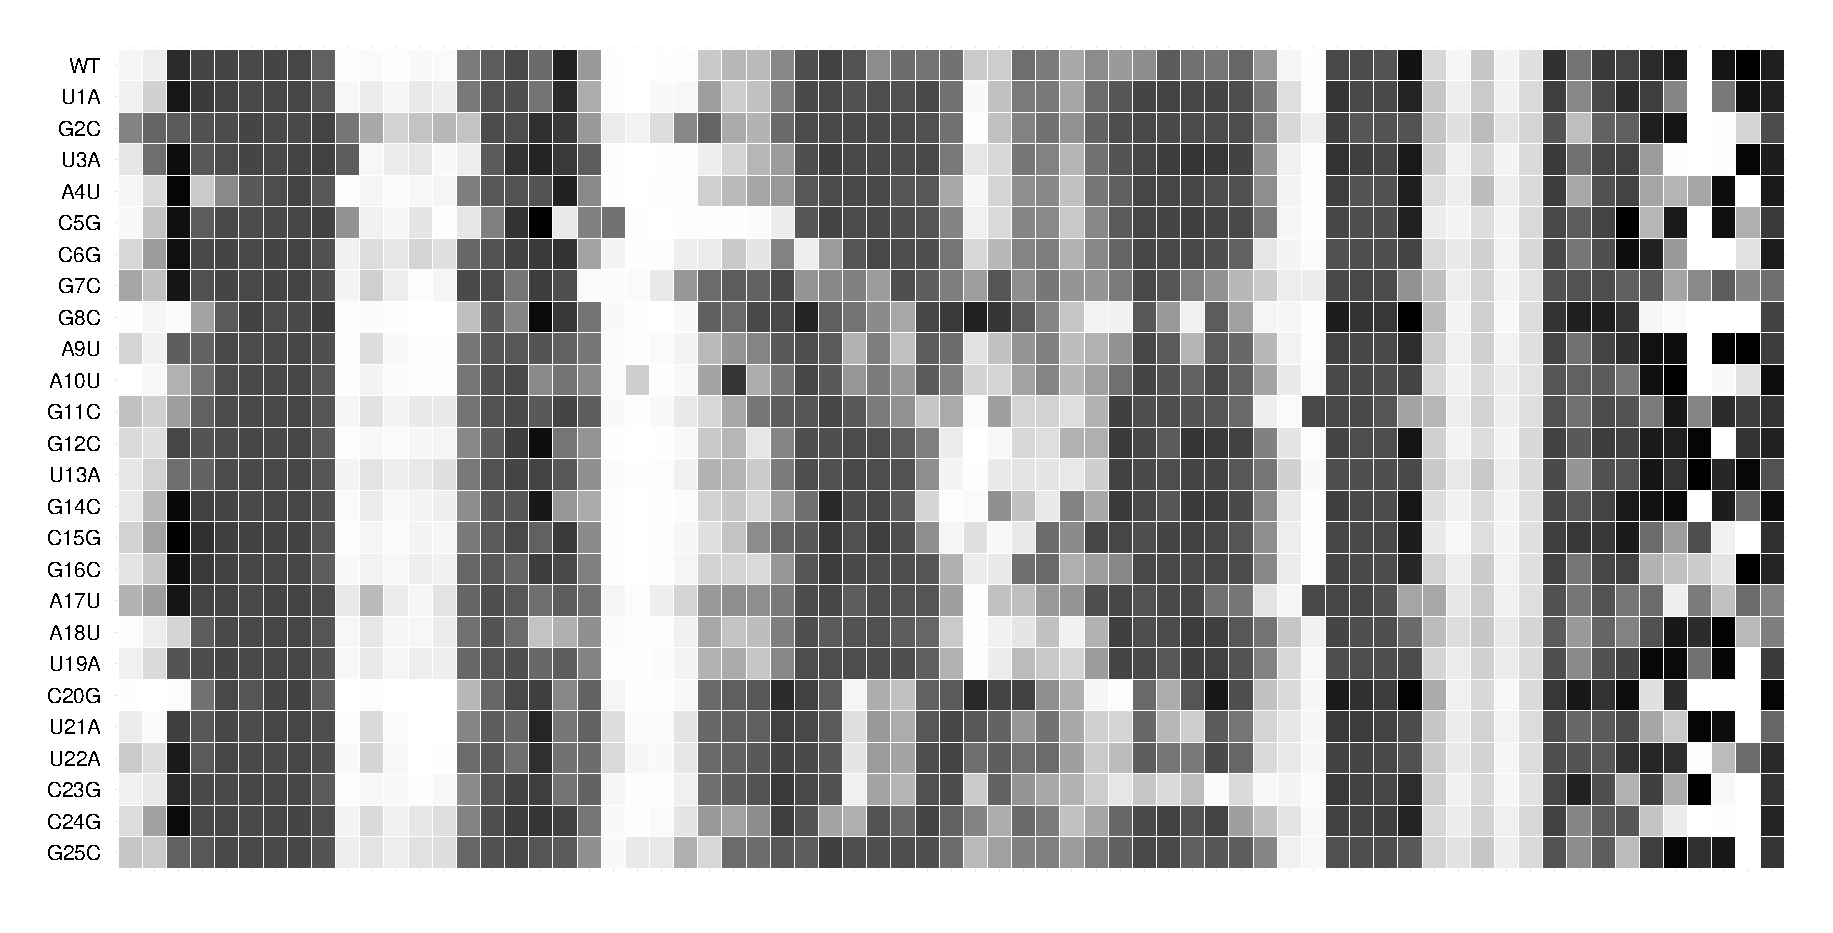
\includegraphics[width=\textwidth]{heatmap.eps}
\caption{Mutate and map experimental outcome. Disruption can be seen
  in rows G7C, G8C, and C20G through C23G.}
\label{fig:heatmap}
\end{figure}

A goal of this analysis is to compare the output of a mutate and map
experiment with the output of Nestor PF. There are a couple obstacles
in the way of this: reactivities, the output of the experiments, are
not normalized on a [0,1] scale, in fact the reactivity is distributed
somewhat like a power law distribution $1/r$. Another is that there is
no direct way to infer clusters from the mutate and map
experiments. To solve these analysis challenges, we developed a
normalization strategy for reactivity and a method of cluster analysis
on the data.

The specific analysis focused on was on a single sequence, the
Hobartner Bistable Switch. 

\subsection{Normalization Strategy}

The central assumption made by our normalization strategy is that the
distribution of reactivities follows the same ranking as partition
function probabilities of pairing. Explicitly, we assume that, for
bases $i$ and $j$, if in terms of partition probability of pairing
$P(i)>P(j)$, then reactivities $r(i) > r(j)$ and vice versa. We also
have a theoretical distribution for the probabilities, $P(i)$. Because
of this, we chose to normalize the reactivities by rank sorting them
and mapping them onto rank sorted partition function probabilities.

\subsection{Cluster Data Analysis}

The mutate and map data from the bistable switch was modeled as
``superpositions'' of two macrostates to get the reactivities of each
mutatant. Specifically, if the two macrostates are $\mu$ and $\nu$,
they each have probabilities $P^\mu_i$ and $P^\nu_i$ for each base $i$
being paired, and then each mutant has a certain probability for each
macrostate $p^\mu_m$ and $p^\nu_n$. Putting the model together looks
something like:
\begin{equation}
\begin{bmatrix}
p^\mu_1 & p^\nu_1 \\
p^\mu_2 & p^\nu_2 \\
\vdots & \vdots \\
p^\mu_m & p^\nu_m
\end{bmatrix}
\begin{bmatrix}
P^\mu_1 & P^\mu_2 & \dots & P^\mu_n \\
P^\nu_1 & P^\nu_2 & \dots & P^\nu_n
\end{bmatrix} + E = 
\begin{bmatrix}
r_{11} & r_{12} & \dots & r_{1n} \\
r_{21} & r_{22} & \dots & r_{2n} \\
\vdots & &\ddots & \vdots \\
r_{m1} & r_{m2} & \dots & r_{mn}
\end{bmatrix},
\end{equation}
where the $r_{mn}$'s are the mapped reactivities and $E$ is the model
error matrix. The parameters, the $p^\mu_m$'s and the $P^\mu_i$'s, are
fit to this model using a boxed gradient descent from the R
\emph{optim} package \cite{byrd1995limited}.

\subsection{Results}

For both reactivity fit and the partition function theory, we classify
pairs above $.25$ probability as predicted, and not predicted
otherwise. Using this analysis I found the around 55\% of base pairs
were properly matched between the SHAPE analysis and Nestor
predictions. This does not seem like much because the prediction
algorithms when compared to crystal structures get better accuracy, of
up to 70\%. However, this is the first time this analysis has been
done, so it is pretty amazing we were able to get any pairs at
all. See Figures \ref{fig:nestResults1} and \ref{fig:nestResults2} to see
how well they match up.
\begin{figure}[t] 
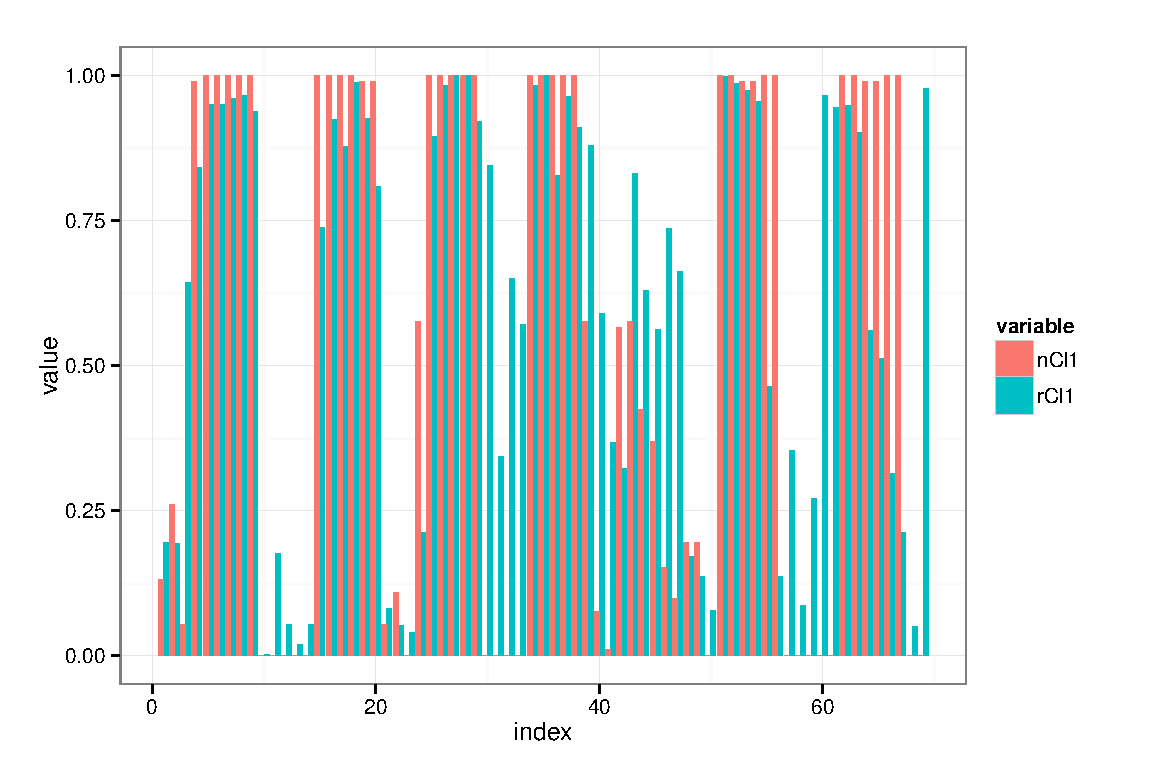
\includegraphics[width=\textwidth]{NestorReactivityPlot1.eps}
\caption{The results of comparing the first cluster results of nestor
  ``nCl1'' against the cluster analysis on SHAPE data ``rCL1''. The x
  axis is base index and the y axis is probability.}
\label{fig:nestResults1}
\end{figure}

\begin{figure}[t]
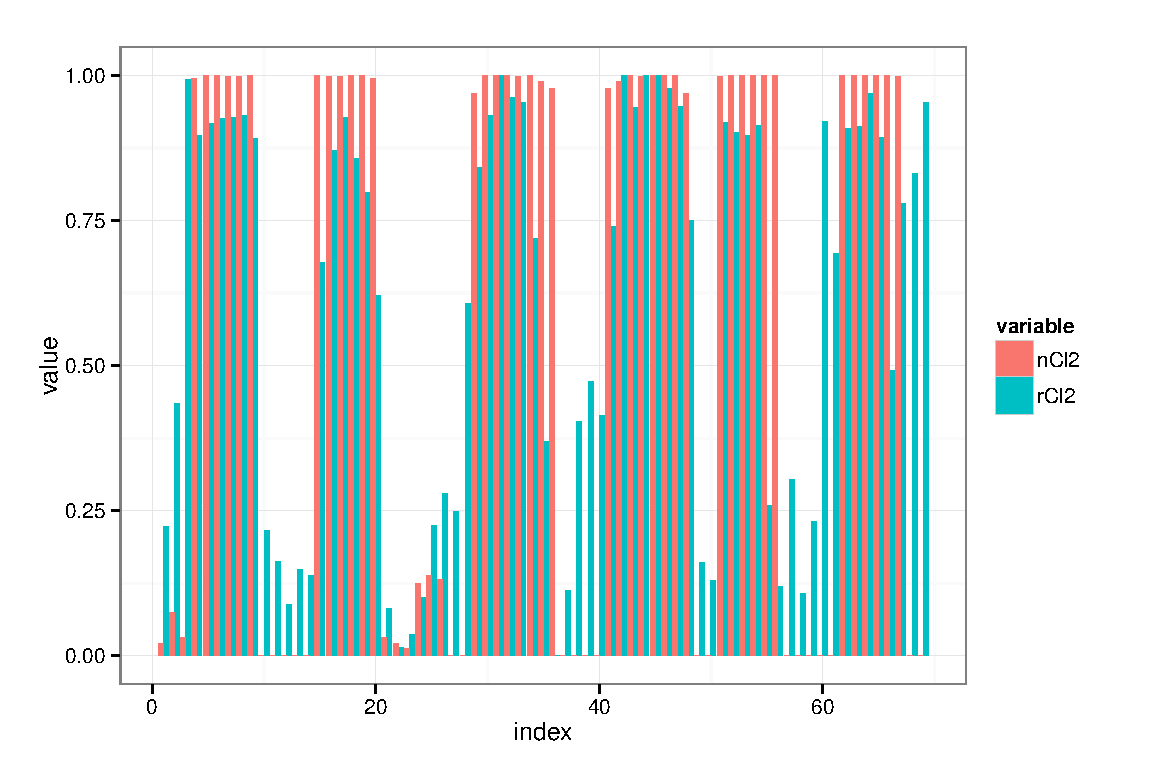
\includegraphics[width=\textwidth]{NestorReactivityPlot2.eps}
\caption{The results of comparing the second cluster results of nestor
  ``nCl2'' against the cluster analysis on SHAPE data ``rCL2''. The x
  axis is base index and the y axis is probability.}
\label{fig:nestResults2}
\end{figure}




